\documentclass[a4paper,10pt]{article}
\usepackage[utf8]{inputenc}
\usepackage{url}
\usepackage{hyperref}
\usepackage{listings}
\usepackage{color}
\usepackage{verbatim}
\definecolor{grey}{rgb}{0.9,0.9,0.9}
\usepackage{boites}
\usepackage{float}
\usepackage{chngpage}
\usepackage{wrapfig}
\usepackage{graphicx}
\usepackage{fancyhdr}
\pagestyle{fancy} % voir si laisse ce style ou pas ?
\lstset{
language=C++,
basicstyle=\footnotesize\fontfamily{pcr},
backgroundcolor=\color{grey},
numbers=left,
numberstyle=\tiny,
numbersep=5pt,
showstringspaces=false,
tabsize=2,
breaklines=true
}


% Title Page
\title{INFO-F404 Operating Systems II - Projet 1}
\author{Chapeaux Thomas\\Dagnely Pierre}

\begin{document}
\maketitle

%%%%%%%%%%%%%%%%%%%%%%%%%%%%%%%%%%%%%%%%%%%%%%%%%%%%%%%%%%%%%%%%%%%%%%%%%%%%%%%%%%%%%%%%%%%%%%%%%%%%%%%%%%%%%%%%%%%%%%%%%%%%%%%%%%%%%%%%%
%%
%%
%%	Intro
%%
%%
%%%%%%%%%%%%%%%%%%%%%%%%%%%%%%%%%%%%%%%%%%%%%%%%%%%%%%%%%%%%%%%%%%%%%%%%%%%%%%%%%%%%%%%%%%%%%%%%%%%%%%%%%%%%%%%%%%%%%%%%%%%%%%%%%%%%%%%%%%
\section{Introduction}

	Le but de ce projet était de construire en C++ un simulateur d'ordonnancement multiprocesseur d'un systèmes de tâches à temps réel via EDF Global ou 		EDF-k, ainsi qu'un générateur de systèmes de tâche permettant de spécifier le nombre de tâches du système ainsi que son utilisation globale.\\		

	Ensuite, il nous était demandé d'utiliser ces modules pour comparer les deux algorithmes (EDF Global et EDF-k) selon le nombre de préemptions, de 			migrations, de cœurs utilisés et d'instants oisifs.

%%%%%%%%%%%%%%%%%%%%%%%%%%%%%%%%%%%%%%%%%%%%%%%%%%%%%%%%%%%%%%%%%%%%%%%%%%%%%%%%%%%%%%%%%%%%%%%%%%%%%%%%%%%%%%%%%%%%%%%%%%%%%%%%%%%%%%%%%
%%
%%
%%	Implémentation
%%
%%
%%%%%%%%%%%%%%%%%%%%%%%%%%%%%%%%%%%%%%%%%%%%%%%%%%%%%%%%%%%%%%%%%%%%%%%%%%%%%%%%%%%%%%%%%%%%%%%%%%%%%%%%%%%%%%%%%%%%%%%%%%%%%%%%%%%%%%%%%%
\section{Choix d'implémentation}

	\subsection{Nature du simulateur}
		Notre simulateur utilise un temps discret (comme vu en cours) et est à pas constant. Il simule le système passé en paramètre avec un nombre de cœur 		choisi par l'utilisateur, mais contient aussi une fonction permettant de calculer ce nombre. La simulation durera le temps maximal nécessaire pour 			effectuer une période complète ($2*PPCM(T_i) + max(O_i)$).

	\subsection{Nature du système}
		Comme demandé par l'énoncé, le simulateur accepte des systèmes périodiques à départ différé et à échéance contrainte. Il ne vérifie pas la 					faisabilité du système avant de commencer, mais s'arrête dés qu'un travail manque son échéance.\\

		En pratique, les systèmes générés sont cependant à échéances implicites.
		En effet, nous avons dans ce cas des systèmes dont on peut calculer la faisabilité ($U_{max} \le 1$) et le nombre de cœurs requis ($\lceil 					U_{globale} \rceil$) sans trop de complexité\footnote{Précisons : Ceci est la solution proposée par Mr Goossens}.

	\subsection{Génération de tâches}
		La génération du système de $n$ tâches avec une utilisation $U_{globale}$ se fait en trois étapes.\\

		Premièrement, on génère les $n$ tâches avec des paramètres aléatoires (distribution uniforme entre deux bornes pour chaque paramètre). Le WCET est 			bien entendu borné par la valeur de l'échéance.\\

		Ensuite, on calcule le facteur d'erreur $F_u = \frac{\Sigma U_i}{U_{globale}}$ et on l'applique à toutes les tâches soit en multipliant le WCET 			soit en	divisant la période (une chance sur deux pour chaque tâche).\\

		Ceci ne nous donne pas encore l'utilisation demandée pour deux raisons : premièrement, le système étant à temps discret, les résultats des 					opérations sont toujours arrondies à l'entier le plus proche ce qui crée des imprécisions. Ensuite, le facteur d'erreur est limité par les 					contraintes logiques des tâches ($wcet \ge 1$, $wcet \le deadline$, etc).\\

		On effectue donc une troisième étape dans laquelle on va, jusqu'à obtenir une utilisation acceptable, sélectionner une tâche au hasard et faire 			varier son wcet ou sa période de 1 pour faire augmenter ou diminuer son utilisation (en fonction de ce qui est nécessaire).\\

		Ce système nous semble générer des systèmes assez variés en un temps raisonnable.

	\subsection{Structures de données}
		Il a été choisi d'utiliser la structure $deque$\footnote{\url{http://www.cplusplus.com/reference/deque/deque/}} de la STL pour le stockage des 				tâches (\verb?tasks?), des travaux actifs, donc entrés dans le système et dont la deadline n'est pas dépassée (\verb?jobs?) et pour les différents 			cœurs (\verb?CPUs?, qui contient des pointeurs vers des éléments de \verb?jobs?).\\

		Les travaux actifs sont également référencés par deux files à priorité de pointeurs vers des travaux : la file \verb?Running?, contenant les 				travaux en cours de calcul par un des cœurs (dont l'élément le plus prioritaire est le travail avec la plus $faible$ priorité), et la file 					\verb?Ready?, contenant tous les autres travaux actifs (dont l'élément le plus prioritaire est le travail avec la plus $grande$ priorité).\\

		On notera qu'il existe deux structures de pointeurs vers les travaux en cours de calcul : la file \verb?Running? et la deque \verb?CPUs?. Ceci est 			dû au fait qu'une file à priorité ne permet pas facilement d'accéder à l'entierté des éléments ou de différencier les différents cœurs (pour le 			compteur de migration).
		
		
	\subsection{Implémentation de EDF-k}
		Après avoir chargé le système (passé en paramètre ou lu sur un fichier), on calcule le nombre minimale de cœurs et le nombre de tâches prioritaires avec la formule : $ m_{min}(T) = \min_{k=1}^n \{  (k-1) + \lceil \frac{U^{(T^{(k+1)})}}{1- U(T_k)}  \rceil \} $.\\
		~\\
		On lance ensuite un simulateur global EDF qu'on a légèrement adapté pour qu'il puisse gérer les jobs prioritaires (\hyperlink{prioriteEDFk}{c.f. chap 3.2} ).\\
		Ainsi quel que soit l'état du système ceux-ci passeront devant les autres jobs et ils auront l'impression d'avoir un processeur chacun.
		
		
	\subsection{Implémentation de global EDF}
		Après avoir chargé le système (passé en paramètres ou lu sur un fichier), on calcule le nombre minimale de cœur avec la formule : $ m_{min} =\lceil 		U_{globale} \rceil$.\\
		~\\
		On lance ensuite le simulateur global EDF. C'est le même que pour EDF-k, mais tous les jobs ayant la même priorité (nulle), celui-ci se comporte alors en "pure" global EDF.

	\subsection{Implémentation du simulateur}
		Voici une version simplifiée de la boucle principale de notre simulateur :
		\fontfamily{pcr}
		\begin{lstlisting}
while (_t < studyInterval) {
	generateNewJobs(_t);
	// scheduling : assign which jobs goes to which CPUs
	while (not _readyJobs.empty()
	and (availableCPUs or JobNeedToBePreempted() )) {
	// The earliest-deadline active job should get a CPU
		if (availableCPUs)
		{
			Job* newJob = _readyJobs.pop();
			_CPUs[firstIdleCPU] = newJob;
			_runningJobs.push(newJob);
		}
		else // all CPUs are busy, preempt the one with the latest deadline
		{
			Job* oldJob = _runningJobs.pop();
			Job* newJob = _readyJobs.pop();
			_CPUs[posOldJob] = newJob;
			_readyJobs.push(oldJob);
			_runningJobs.push(newJob);
			preemption_counter++;
		}
	}

	// CPUs
	for (unsigned int i = 0; i < _CPUs.size(); ++i)
	{
		if (_CPUs[i] != NULL)
		{
			// compute jobs in CPUs
			if (_CPUs[i]->getLastCPU_Id() != (int) i)
				++migration_counter;
			_CPUs[i]->giveCPU(_deltaT, i);
			
			// check if a job is done
			if (_CPUs[i]->getComputationLeft() == 0)
				_CPUs[i] = NULL;
			else
				++idle_time_counter;
		}
	}
	// advance time
	_t += _deltaT;
	cleanAndCheckJobs(_t);
}
\end{lstlisting}
\fontfamily{}

		\paragraph*{Récoltes de statistiques}~\\

			Notre simulateur renvoie l'intervalle d'étude, le nombre de préemptions, d'instants oisifs et de migrations apparues au cours de la simulation.

		
		%Nous avons récoltés les données suivantes :

		%\begin{description}
		 %\item[Préemption :] Un cœur change de travail alors que le précédent n'était pas terminé.
		 %\item[Migration :] Un travail reprend son exécution sur un cœur différent du précédent.
		 %\item[Instant oisif :] Un cœur n'a pas de travail pour cet instant. Si plusieurs cœurs sont oisifs on augmente le compte de ce nombre de cœurs.
		 %\item[Nombres de cœurs :] Le nombre de cœurs que le simulateur a prévu pour le système, même si certains n'ont jamais été utilisés.
		%\end{description}
	
	\subsection{Implémentation du comparateur}
		Nous avons crée un comparateur lançant deux types de comparaisons, en fonction de ses paramètres.
		\begin{enumerate}
			\item \verb?./globalEDFvsEDF-k -u utilisationVoulue -n nombreDeCœur -t nombreDeTests?
					On compare alors EDF-k et global EDF pour sur des systèmes correspondants.\\
					On lance donc successivement TaskGenerator puis simGlobalEDF et simEDF-k, mais sans passer par des fichiers textes, ils se passent le système et les différents paramètres directement.
			\item \verb?./globalEDFvsEDF-k [sans parametres]?
					On compare ici EDF-k et global EDF pour différentes valeurs d'utilisation et de nombre de tâches à des fins de statistiques.\\
					On essaye des utilisations de (30-50-70-90-110-130-150) pour des systèmes de (5-10-15-20) tâches.\\
					Le résultat est affiché et stocké dans un fichier "statistics.txt"
		\end{enumerate}
		
		
%%%%%%%%%%%%%%%%%%%%%%%%%%%%%%%%%%%%%%%%%%%%%%%%%%%%%%%%%%%%%%%%%%%%%%%%%%%%%%%%%%%%%%%%%%%%%%%%%%%%%%%%%%%%%%%%%%%%%%%%%%%%%%%%%%%%%%%%%
%%
%%
%%	difficultés rencontrées
%%
%%
%%%%%%%%%%%%%%%%%%%%%%%%%%%%%%%%%%%%%%%%%%%%%%%%%%%%%%%%%%%%%%%%%%%%%%%%%%%%%%%%%%%%%%%%%%%%%%%%%%%%%%%%%%%%%%%%%%%%%%%%%%%%%%%%%%%%%%%%%%
\section{Difficultés rencontrées}

	\subsection{Intervalle d'étude}

		Les périodes des tâches sont générées aléatoirement. Hors, elles vont avoir une très grande influence sur l'intervalle d'étude du simulateur vu que 		celui-ci est égal à $PPCM(T_i)+ max(O_i)$. Des périodes tirées aléatoirement peuvent très vite rendre le PPCM relativement grand, jusqu'au point où 		le temps de calcul devient inacceptable.

		Ce problème a été réglé en donnant 19 valeurs de période possibles (dont le PPCM est connu et acceptable) et en choisissant pour chaque tâche une 			de ses valeurs.\\

		Les valeurs choisies sont : {2, 3, 5, 6, 8, 9, 10, 12, 14, 15, 16, 18, 20, 22, 24, 25, 28, 30, 32}, leur PPCM est 554400.

	\subsection{Priorité en EDF-k}\hypertarget{prioriteEDFk}{}

		La principale difficulté de EDF-k est la gestion des tâches prioritaires.\\
		La méthode vue en cours consistait à mettre les deadlines de ces tâches à $- \infty$. mais notre implémentation du simulateur utilise fréquemment ces deadlines pour divers calculs (tester l'ordonnancabilité du système, ...) et la gestion de deadline à $- \infty$ aurait rendu notre code trop complexe.\\
		~\\
		Il nous a donc semblé plus simple de rajouter un paramètre booléen "priority" aux tâches (et donc à leurs jobs), ainsi on ne doit se préoccuper de la priorité qu'à deux endroits :
		\begin{enumerate}
			\item Lors du tri des priority\_queue ready et running, en modifiant le comparateur EDFcomp pour que les jobs prioritaires arrivent au sommet de ready (ainsi ils sont toujours exécuté en premier) et en bas de running (ainsi on regarde prioritairement les autres jobs en cas de préemption).\\
			\item Lors du choix des jobs a préempter, on utilise la méthode "JobNeedToBePreempted()" qui regarde les sommets de ready et running pour définir si une préemption est nécessaire.\\
				S'il y a des jobs prioritaires, ils sont alors privilégiés (ont leur attribue un cœur ou les laisse terminer leur job), sinon on se base sur les deadlines.
		\end{enumerate}
		Ainsi le système peut fonctionner avec des jobs prioritaires, ou sans jobs prioritaires, devenant alors un simulateur global EDF.

%%%%%%%%%%%%%%%%%%%%%%%%%%%%%%%%%%%%%%%%%%%%%%%%%%%%%%%%%%%%%%%%%%%%%%%%%%%%%%%%%%%%%%%%%%%%%%%%%%%%%%%%%%%%%%%%%%%%%%%%%%%%%%%%%%%%%%%%%
%%
%%
%%	Résultat
%%
%%
%%%%%%%%%%%%%%%%%%%%%%%%%%%%%%%%%%%%%%%%%%%%%%%%%%%%%%%%%%%%%%%%%%%%%%%%%%%%%%%%%%%%%%%%%%%%%%%%%%%%%%%%%%%%%%%%%%%%%%%%%%%%%%%%%%%%%%%%%%
\section{Résultats}

 	En se basant sur notre comparateur, on peut déjà analyser assez finement les différences entre global EDF et EDF-k.\\
	
	\paragraph*{Nombre de cœurs}~\\
		Quelque soit le nombre de tâches, jusqu'à une utilisation de 70, ils utilisent touss deux un seul cœur.
		Mais passez ce cap, en moyenne global EDF commence à utiliser de plus en plus de cœurs tandis que EDF-k reste stable.\\
		~\\
		EDF-k est donc plus intéressant pour des système avec une plus grosse utilisation.
		
	\paragraph*{Nombre de préemptions et migrations}~\\

		Quelque soit l'utilisation et le nombre de tâches, EDF-k nécessite en moyenne plus de préemptions, mais moins (voir pas) de migrations que global EDF.\\
		Mais pour de grandes utilisations (et nombre de tâches) on peut avoir des différences significatives, sans qu'une tendance ne se fasse jour.
		
	\paragraph*{Intervalles d'étude}~\\
		Pour de petites utilisations, les intervalles d'études sont assez proches, mais pour de grandes utilisations (et nombre de tâches) on peut avoir des différences significatives, sans qu'une tendance ne se fasse jour.
		

	\paragraph*{Nombre d'instants oisifs}~\\
		Quelque soit l'utilisation et le nombre de tâches, EDF-k et global EDF ont peu ou prou le même nombre d'instants oisifs.
		
	\paragraph*{Nombre de systèmes ordonnancés}~\\
		Quelque soit l'utilisation et le nombre de tâches, global EDF ordonnance plus de systèmes qu'EDF-k.


%%%%%%%%%%%%%%%%%%%%%%%%%%%%%%%%%%%%%%%%%%%%%%%%%%%%%%%%%%%%%%%%%%%%%%%%%%%%%%%%%%%%%%%%%%%%%%%%%%%%%%%%%%%%%%%%%%%%%%%%%%%%%%%%%%%%%%%%%
%%
%%
%%	Appendice
%%
%%
%%%%%%%%%%%%%%%%%%%%%%%%%%%%%%%%%%%%%%%%%%%%%%%%%%%%%%%%%%%%%%%%%%%%%%%%%%%%%%%%%%%%%%%%%%%%%%%%%%%%%%%%%%%%%%%%%%%%%%%%%%%%%%%%%%%%%%%%%%
\pagebreak
\section{Appendice}
	
	
	  	
	 \subsection{Diagramme du programme}
		\begin{figure}[H] \hspace*{-2cm} 
    	\centering
   		  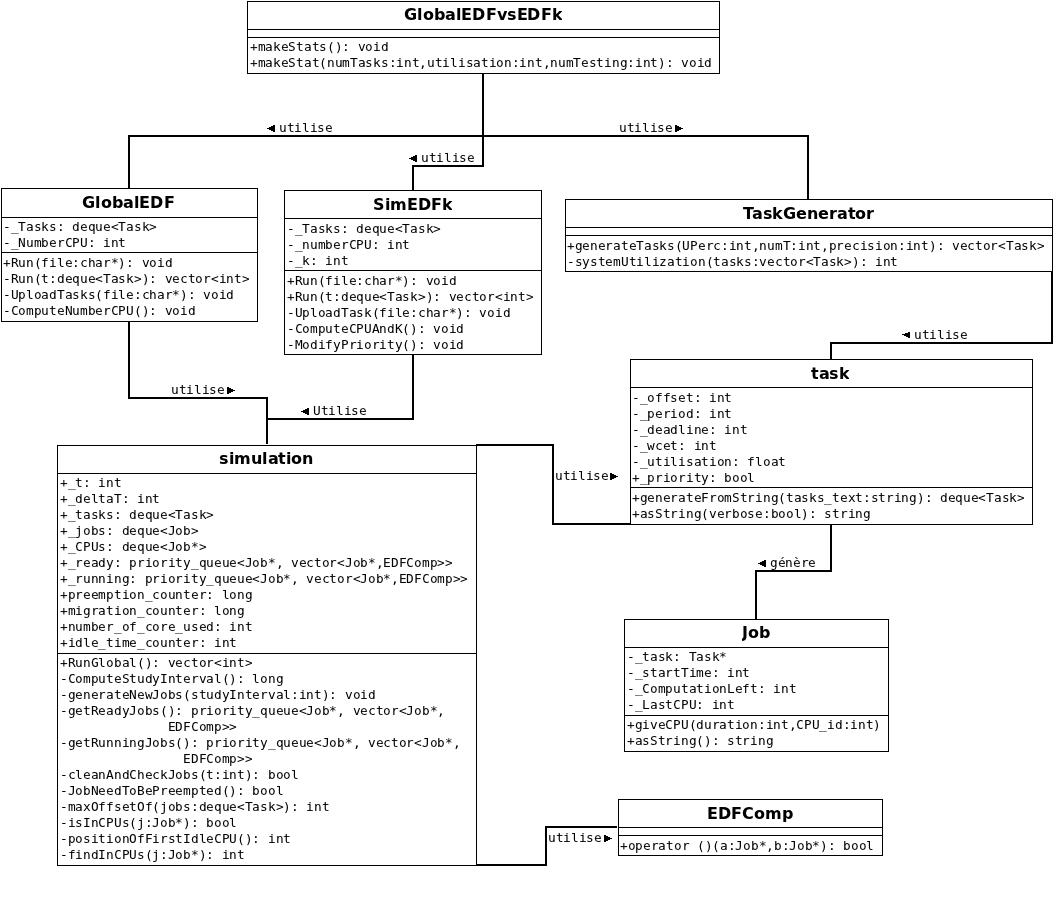
\includegraphics[width=300pt]{DiagUML.jpeg} 
			%\caption{titre}
			%\label{image-label}
	  	\end{figure}
	  
	 \subsection{Output des programmes}
		\begin{figure}[H] \hspace*{-2cm} 
    	\centering
   		  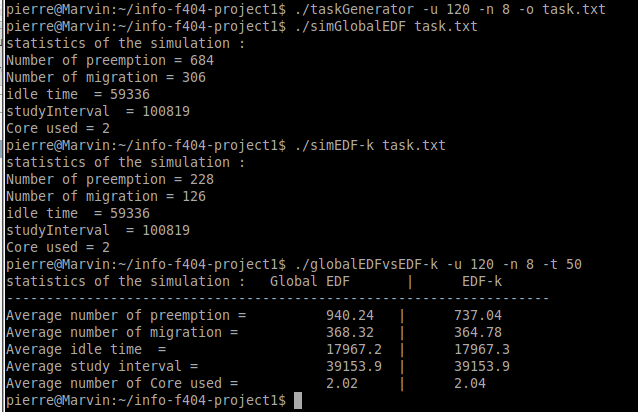
\includegraphics[width=250pt]{output3.png} 
			%\caption{titre}
			%\label{image-label}
	  	\end{figure}
	  	
	  
	 \subsection{Statistiques du comparateur}
		\begin{figure}[H] \hspace*{-2cm} 
    	\centering
   		  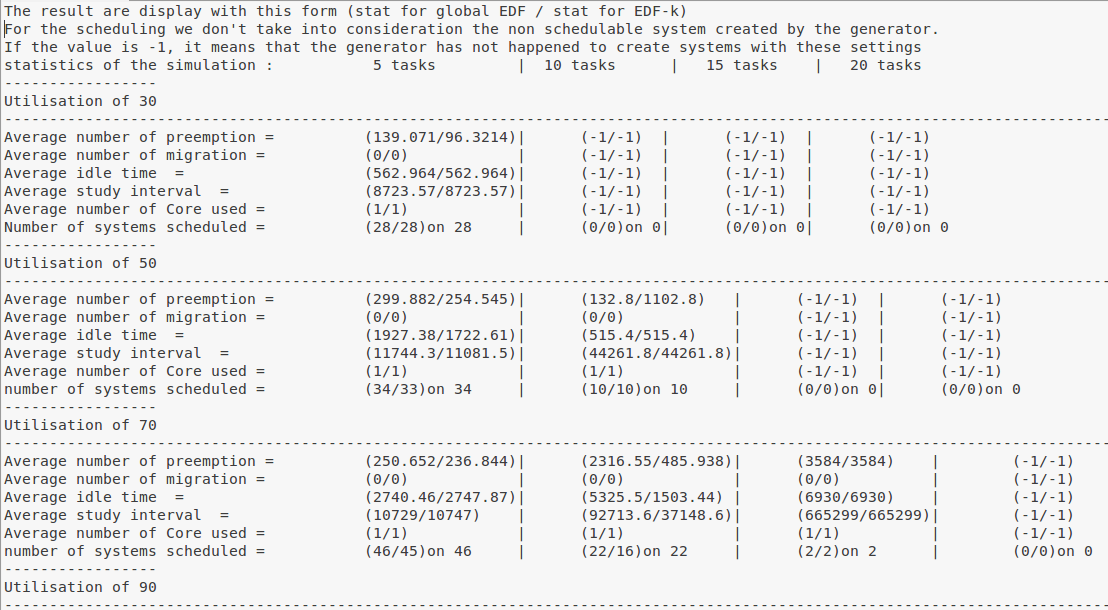
\includegraphics[width=300pt]{stat2.png} 
			%\caption{titre}
			%\label{image-label}
	  	\end{figure}


		Les résultats sont affichés sous la forme (résultat pour global EDF/ résultat pour EDF-k)\\
		Ces statistiques sont générée en produisant (ou en essayant de produire) 50 systèmes respectant les paramètres correspondants.\\
		Cependant il peut arriver que le générateur n'arrive pas à créer un système viable ou que le simulateur n'arrive pas à ordonnancer ce système.\\
		C'est représenter par la ligne "Number of systems scheduled", dont les résultats ont la forme :\\
		(nombre de système ordonnancer par global EDF / par EDF-k) sur le nombre de système créé par le générateur.\\
		~\\
		Si aucun système n'a été créer par le générateur ou n'est ordonnancable, alors les valeurs sont mises à -1.

\leftskip -2cm
{
	  	\paragraph*{Utilisation de 30}~\\
	  	\begin{tabular}{|c|c|c|c|c|} \hline
	  	 &	 	 5 tasks 	 &  10 tasks 	  &   15 tasks 	 &   20 tasks 	\\ \hline
Average number of preemption & 	 	(139.071/96.3214)& 	(-1/-1)	 & 	(-1/-1)	 & 	(-1/-1) \\ \hline
Average number of migration & 		(0/0)	 	 & 	(-1/-1)	 & 	(-1/-1)	 & 	(-1/-1) \\ \hline
Average idle time  & 			(562.964/562.964)& 	(-1/-1)	 & 	(-1/-1)	 & 	(-1/-1) \\ \hline
Average study interval  & 		(8723.57/8723.57)& 	(-1/-1)	 & 	(-1/-1)	 & 	(-1/-1) \\ \hline
Average number of Core used &  	 	(1/1)	 	 & 	(-1/-1)	& 	(-1/-1)	 & 	(-1/-1) \\ \hline
Number of systems scheduled &  	 	(28/28)sur 28	 & 	(0/0)sur 0& 	(0/0)sur 0& 	(0/0)sur 0 \\ \hline
\end{tabular}

\paragraph*{Utilisation de 50}~\\
	  	\begin{tabular}{|c|c|c|c|c|} \hline
	  	 &	 	 5 tasks 	 &  10 tasks 	  &   15 tasks 	 &   20 tasks 	\\ \hline
Average number of preemption  & 	 	(299.882/254.545) & 	(132.8/1102.8)	  & 	(-1/-1)	  & 	(-1/-1)\\ \hline
Average number of migration  & 		(0/0)	 	  & 	(0/0)	          & 	(-1/-1)	  & 	(-1/-1)\\ \hline
Average idle time   & 			(1927.38/1722.61) & 	(515.4/515.4)     & 	(-1/-1)	 & 	(-1/-1)\\ \hline
Average study interval   & 		(11744.3/11081.5) & 	(44261.8/44261.8) & 	(-1/-1)	  &	(-1/-1)\\ \hline
Average number of Core used  &  	 	(1/1)	 	  & 	(1/1)	      	  & 	(-1/-1)	  & 	(-1/-1)\\ \hline
number of systems scheduled  &  	 	(34/33)sur 34	  & 	(10/10)sur 10  	  & 	(0/0)sur 0 & 	(0/0)sur 0\\ \hline
\end{tabular}
\paragraph*{Utilisation de 70}~\\
	  	\begin{tabular}{|c|c|c|c|c|} \hline
	  	 &	 	 5 tasks 	 &  10 tasks 	  &   15 tasks 	 &   20 tasks 	\\ \hline
Average number of preemption & 	 	(250.652/236.844)& 	(2316.55/485.938)& 	(3584/3584)    & 	(-1/-1)\\ \hline
Average number of migration&		(0/0)	 	& 	(0/0)	 	& 	(0/0)	       & 	(-1/-1)\\ \hline
Average idle time  &			(2740.46/2747.87)&	(5325.5/1503.44) & 	(6930/6930)    & 	(-1/-1)\\ \hline
Average study interval & 		(10729/10747)	 & 	(92713.6/37148.6)& 	(665299/665299)& 	(-1/-1)\\ \hline
Average number of Core used &  	 	(1/1)	 	 & 	(1/1)	 	& 	(1/1)	      & 	(-1/-1)\\ \hline
number of systems scheduled &  	 	(46/45)sur 46	 & 	(22/16)sur 22	 &	(2/2)sur 2      & 	(0/0)sur 0\\ \hline
\end{tabular}
\paragraph*{Utilisation de 90}~\\
	  	\begin{tabular}{|c|c|c|c|c|} \hline
	  	 &	 	 5 tasks 	 &  10 tasks 	  &   15 tasks 	 &   20 tasks 	\\ \hline
Average number of preemption & 	 	(290.735/254.255)	& 	(1558.19/5303.62)& 	(2793.67/17722)	 & 	(-1/-1)\\ \hline
Average number of migration & 		(0.857143/0)	 	 & 	(154.857/0)	&	(1414.67/0)	& 	(-1/-1)\\ \hline
Average idle time  &			(4056.86/4162.34)	 & 	(30420.1/30420)	 & 	(41400.7/61777)	& 	(-1/-1)\\ \hline
Average study interval &		(8843.27/9055.47)	 & 	(148017/148017)	 &	(464258/693018)	 & 	(-1/-1)\\ \hline
Average number of Core used &  	 	(1.18367/1)	 	&	(1.52381/1)	 & 	(1.33333/1)	 & 	(-1/-1)\\ \hline
number of systems scheduled &  	 	(49/47)sur 49	 	& 	(21/21)sur 22	& 	(3/2)sur 3	& 	(0/0)sur 0\\ \hline
\end{tabular}
\paragraph*{Utilisation de 110}~\\
	  	\begin{tabular}{|c|c|c|c|c|} \hline
	  	 &	 	 5 tasks 	 &  10 tasks 	  &   15 tasks 	 &   20 tasks 	\\ \hline
Average number of preemption &	 	(134.9/147.439)	 	 & 	(1555.37/3701.29)& 	(3028.36/19065.4)& 	(18/179)\\ \hline
Average number of migration & 		(4.12/0)	 	 & 	(253.086/0)	& 	(1611.36/0)	& 	(12/0)\\ \hline
Average idle time &			(1952.3/2021.07)	 & 	(20079/20562.1)	& 	(56705.6/63785.1)&	(336.5/336.5)\\ \hline
Average study interval &		(4085.9/4435.85)	 & 	(82489.4/89385)	 & 	(379973/415578)	& 	(564499/564499)\\ \hline
Average number of Core used & 	 	(1.58/1)	 	 & 	(1.74286/1)	 & 	(2/1)	 	& 	(2/1)\\ \hline
number of systems scheduled &  	 	(50/41)sur 50	 	&	(35/28)sur 35	& 	(14/12)sur 14	&	(2/2)sur 2\\ \hline
\end{tabular}
\paragraph*{Utilisation de 130}~\\
	  	\begin{tabular}{|c|c|c|c|c|} \hline
	  	 &	 	 5 tasks 	 &  10 tasks 	  &   15 tasks 	 &   20 tasks 	\\ \hline
Average number of preemption&	 	(67.1/265.4)   	&	(1336.77/5378.79)& 	(4484.7/15784.7) & 	(19781.2/12188)\\ \hline
Average number of migration & 		(33.62/0)      & 	(660.977/0)	 & 	(2783.05/0)	 & 	(8184.5/0)\\ \hline
Average idle time  & 			(4155.7/3317.4)	 & 	(22398.9/25310.2)& 	(63951.4/42576.7)&	(51123/44422)\\ \hline
Average study interval  & 		(6630.68/5948.14)& 	(64000.1/74866.3)& 	(252421/252910)	 &	(413299/221779)\\ \hline
Average number of Core used & 	 	(2/1)	 	 & 	(2/1)		 & 	(2/1)	 	 & 	(2/1)\\ \hline
number of systems scheduled & 	 	(50/35)sur 50	& 	(44/33)sur 44	& 	(20/14)sur 20	 & 	(4/1)sur 4\\ \hline
\end{tabular}
\paragraph*{Utilisation de 150}~\\
	\begin{tabular}{|c|c|c|c|c|} \hline
	  	 &	 	 5 tasks 	 &  10 tasks 	  &   15 tasks 	 &   20 tasks 	\\ \hline
Average number of preemption & 	 	(317.18/44.5)	& 	(3663.46/1649.63)& 	(5745.63/11241)	 &	(11845.7/727)\\ \hline
Average number of migration & 		(177.2/0)	& 	(1893.92/0)	 & 	(2808.67/0)	& 	(6541.78/0)\\ \hline
Average idle time  & 			(10262.2/555.25) & 	(49392.2/19220.1)& 	(58701.3/30494.5)& 	(89861.8/2650.33)\\ \hline
Average study interval  & 		(9648.22/1171.94)& 	(75048.2/45472.4)& 	(188352/137602)	 & 	(537992/50418.7)\\ \hline
Average number of Core used &  	 	(2/1)	 	 & 	(2/1)		& 	(2/1)	 	& 	(2/1)\\ \hline
number of systems scheduled & 	 	(50/16)sur 50	& 	(48/27)sur 48	&	(27/17)sur 27	&	(9/3)sur 9	\\ \hline
\end{tabular}
}
	

\end{document}          
